\documentclass[]{book}
\usepackage{lmodern}
\usepackage{amssymb,amsmath}
\usepackage{ifxetex,ifluatex}
\usepackage{fixltx2e} % provides \textsubscript
\ifnum 0\ifxetex 1\fi\ifluatex 1\fi=0 % if pdftex
  \usepackage[T1]{fontenc}
  \usepackage[utf8]{inputenc}
\else % if luatex or xelatex
  \ifxetex
    \usepackage{mathspec}
  \else
    \usepackage{fontspec}
  \fi
  \defaultfontfeatures{Ligatures=TeX,Scale=MatchLowercase}
\fi
% use upquote if available, for straight quotes in verbatim environments
\IfFileExists{upquote.sty}{\usepackage{upquote}}{}
% use microtype if available
\IfFileExists{microtype.sty}{%
\usepackage{microtype}
\UseMicrotypeSet[protrusion]{basicmath} % disable protrusion for tt fonts
}{}
\usepackage[margin=1in]{geometry}
\usepackage{hyperref}
\hypersetup{unicode=true,
            pdftitle={A Compendium Of Statistics Questions},
            pdfauthor={Richard White},
            pdfborder={0 0 0},
            breaklinks=true}
\urlstyle{same}  % don't use monospace font for urls
\usepackage{natbib}
\bibliographystyle{apalike}
\usepackage{color}
\usepackage{fancyvrb}
\newcommand{\VerbBar}{|}
\newcommand{\VERB}{\Verb[commandchars=\\\{\}]}
\DefineVerbatimEnvironment{Highlighting}{Verbatim}{commandchars=\\\{\}}
% Add ',fontsize=\small' for more characters per line
\usepackage{framed}
\definecolor{shadecolor}{RGB}{248,248,248}
\newenvironment{Shaded}{\begin{snugshade}}{\end{snugshade}}
\newcommand{\KeywordTok}[1]{\textcolor[rgb]{0.13,0.29,0.53}{\textbf{{#1}}}}
\newcommand{\DataTypeTok}[1]{\textcolor[rgb]{0.13,0.29,0.53}{{#1}}}
\newcommand{\DecValTok}[1]{\textcolor[rgb]{0.00,0.00,0.81}{{#1}}}
\newcommand{\BaseNTok}[1]{\textcolor[rgb]{0.00,0.00,0.81}{{#1}}}
\newcommand{\FloatTok}[1]{\textcolor[rgb]{0.00,0.00,0.81}{{#1}}}
\newcommand{\ConstantTok}[1]{\textcolor[rgb]{0.00,0.00,0.00}{{#1}}}
\newcommand{\CharTok}[1]{\textcolor[rgb]{0.31,0.60,0.02}{{#1}}}
\newcommand{\SpecialCharTok}[1]{\textcolor[rgb]{0.00,0.00,0.00}{{#1}}}
\newcommand{\StringTok}[1]{\textcolor[rgb]{0.31,0.60,0.02}{{#1}}}
\newcommand{\VerbatimStringTok}[1]{\textcolor[rgb]{0.31,0.60,0.02}{{#1}}}
\newcommand{\SpecialStringTok}[1]{\textcolor[rgb]{0.31,0.60,0.02}{{#1}}}
\newcommand{\ImportTok}[1]{{#1}}
\newcommand{\CommentTok}[1]{\textcolor[rgb]{0.56,0.35,0.01}{\textit{{#1}}}}
\newcommand{\DocumentationTok}[1]{\textcolor[rgb]{0.56,0.35,0.01}{\textbf{\textit{{#1}}}}}
\newcommand{\AnnotationTok}[1]{\textcolor[rgb]{0.56,0.35,0.01}{\textbf{\textit{{#1}}}}}
\newcommand{\CommentVarTok}[1]{\textcolor[rgb]{0.56,0.35,0.01}{\textbf{\textit{{#1}}}}}
\newcommand{\OtherTok}[1]{\textcolor[rgb]{0.56,0.35,0.01}{{#1}}}
\newcommand{\FunctionTok}[1]{\textcolor[rgb]{0.00,0.00,0.00}{{#1}}}
\newcommand{\VariableTok}[1]{\textcolor[rgb]{0.00,0.00,0.00}{{#1}}}
\newcommand{\ControlFlowTok}[1]{\textcolor[rgb]{0.13,0.29,0.53}{\textbf{{#1}}}}
\newcommand{\OperatorTok}[1]{\textcolor[rgb]{0.81,0.36,0.00}{\textbf{{#1}}}}
\newcommand{\BuiltInTok}[1]{{#1}}
\newcommand{\ExtensionTok}[1]{{#1}}
\newcommand{\PreprocessorTok}[1]{\textcolor[rgb]{0.56,0.35,0.01}{\textit{{#1}}}}
\newcommand{\AttributeTok}[1]{\textcolor[rgb]{0.77,0.63,0.00}{{#1}}}
\newcommand{\RegionMarkerTok}[1]{{#1}}
\newcommand{\InformationTok}[1]{\textcolor[rgb]{0.56,0.35,0.01}{\textbf{\textit{{#1}}}}}
\newcommand{\WarningTok}[1]{\textcolor[rgb]{0.56,0.35,0.01}{\textbf{\textit{{#1}}}}}
\newcommand{\AlertTok}[1]{\textcolor[rgb]{0.94,0.16,0.16}{{#1}}}
\newcommand{\ErrorTok}[1]{\textcolor[rgb]{0.64,0.00,0.00}{\textbf{{#1}}}}
\newcommand{\NormalTok}[1]{{#1}}
\usepackage{longtable,booktabs}
\usepackage{graphicx,grffile}
\makeatletter
\def\maxwidth{\ifdim\Gin@nat@width>\linewidth\linewidth\else\Gin@nat@width\fi}
\def\maxheight{\ifdim\Gin@nat@height>\textheight\textheight\else\Gin@nat@height\fi}
\makeatother
% Scale images if necessary, so that they will not overflow the page
% margins by default, and it is still possible to overwrite the defaults
% using explicit options in \includegraphics[width, height, ...]{}
\setkeys{Gin}{width=\maxwidth,height=\maxheight,keepaspectratio}
\IfFileExists{parskip.sty}{%
\usepackage{parskip}
}{% else
\setlength{\parindent}{0pt}
\setlength{\parskip}{6pt plus 2pt minus 1pt}
}
\setlength{\emergencystretch}{3em}  % prevent overfull lines
\providecommand{\tightlist}{%
  \setlength{\itemsep}{0pt}\setlength{\parskip}{0pt}}
\setcounter{secnumdepth}{5}
% Redefines (sub)paragraphs to behave more like sections
\ifx\paragraph\undefined\else
\let\oldparagraph\paragraph
\renewcommand{\paragraph}[1]{\oldparagraph{#1}\mbox{}}
\fi
\ifx\subparagraph\undefined\else
\let\oldsubparagraph\subparagraph
\renewcommand{\subparagraph}[1]{\oldsubparagraph{#1}\mbox{}}
\fi

%%% Use protect on footnotes to avoid problems with footnotes in titles
\let\rmarkdownfootnote\footnote%
\def\footnote{\protect\rmarkdownfootnote}

%%% Change title format to be more compact
\usepackage{titling}

% Create subtitle command for use in maketitle
\newcommand{\subtitle}[1]{
  \posttitle{
    \begin{center}\large#1\end{center}
    }
}

\setlength{\droptitle}{-2em}
  \title{A Compendium Of Statistics Questions}
  \pretitle{\vspace{\droptitle}\centering\huge}
  \posttitle{\par}
  \author{Richard White}
  \preauthor{\centering\large\emph}
  \postauthor{\par}
  \predate{\centering\large\emph}
  \postdate{\par}
  \date{2017-06-07}

\usepackage{booktabs}
\usepackage{amsthm}
\makeatletter
\def\thm@space@setup{%
  \thm@preskip=8pt plus 2pt minus 4pt
  \thm@postskip=\thm@preskip
}
\makeatother

\usepackage{amsthm}
\newtheorem{theorem}{Theorem}[chapter]
\newtheorem{lemma}{Lemma}[chapter]
\theoremstyle{definition}
\newtheorem{definition}{Definition}[chapter]
\newtheorem{corollary}{Corollary}[chapter]
\newtheorem{proposition}{Proposition}[chapter]
\theoremstyle{definition}
\newtheorem{example}{Example}[chapter]
\theoremstyle{remark}
\newtheorem*{remark}{Remark}
\begin{document}
\maketitle

{
\setcounter{tocdepth}{1}
\tableofcontents
}
\chapter{Purpose}\label{purpose}

This is a compendium of commonly asked statistical questions.

\chapter{Introduction}\label{intro}

You can label chapter and section titles using \texttt{\{\#label\}}
after them, e.g., we can reference Chapter \ref{intro}. If you do not
manually label them, there will be automatic labels anyway, e.g., .

Figures and tables with captions will be placed in \texttt{figure} and
\texttt{table} environments, respectively.

\begin{Shaded}
\begin{Highlighting}[]
\KeywordTok{par}\NormalTok{(}\DataTypeTok{mar =} \KeywordTok{c}\NormalTok{(}\DecValTok{4}\NormalTok{, }\DecValTok{4}\NormalTok{, .}\DecValTok{1}\NormalTok{, .}\DecValTok{1}\NormalTok{))}
\KeywordTok{plot}\NormalTok{(pressure, }\DataTypeTok{type =} \StringTok{'b'}\NormalTok{, }\DataTypeTok{pch =} \DecValTok{19}\NormalTok{)}
\end{Highlighting}
\end{Shaded}

\begin{figure}

{\centering 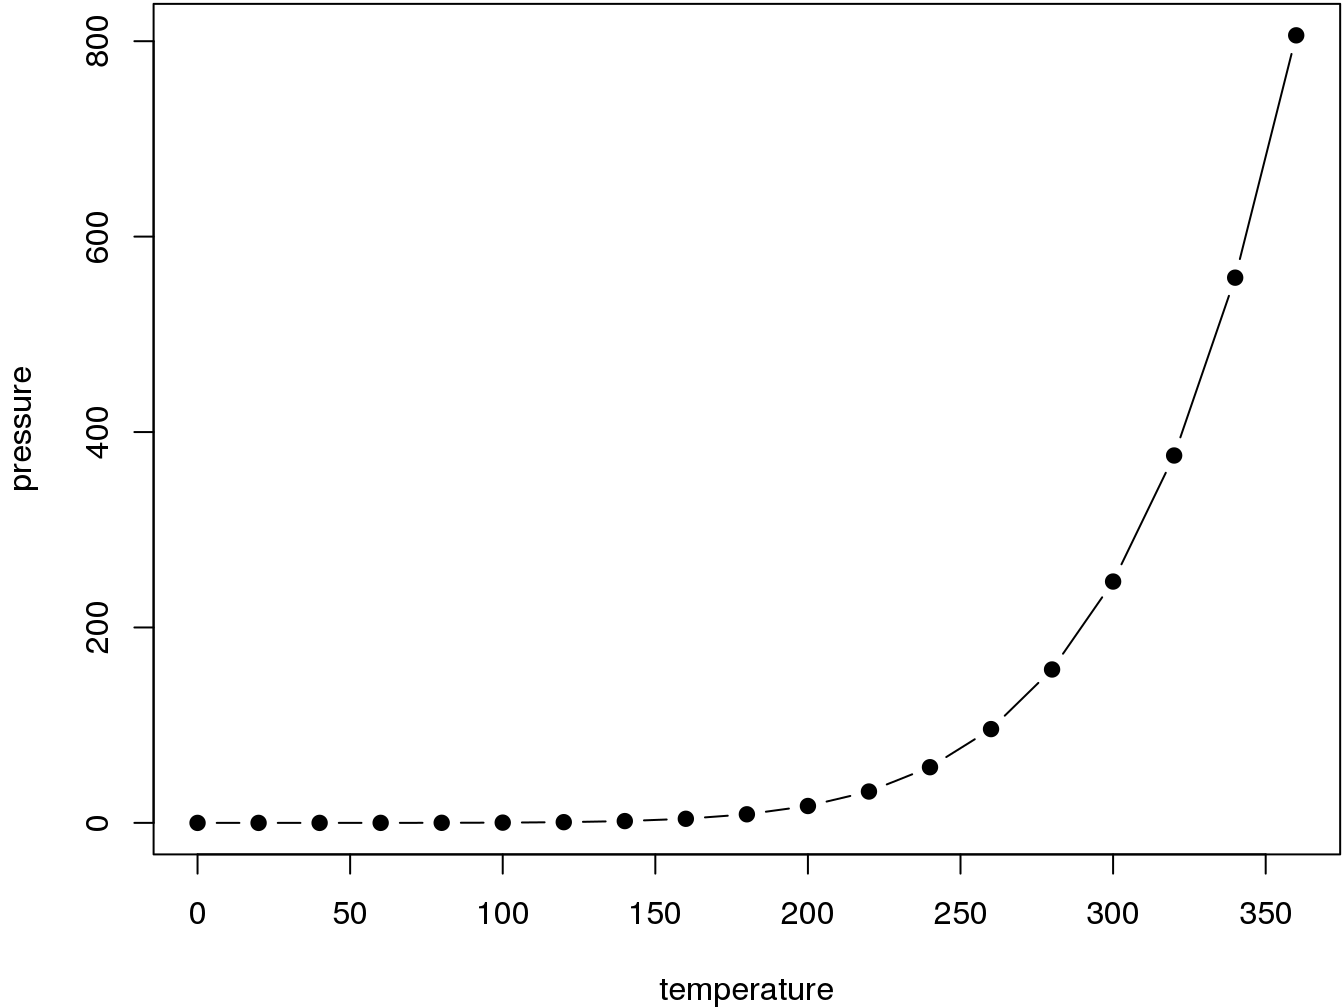
\includegraphics[width=0.8\linewidth]{a-compendium-of-statistics-questions_files/figure-latex/nice-fig-1} 

}

\caption{Here is a nice figure!}\label{fig:nice-fig}
\end{figure}

Reference a figure by its code chunk label with the \texttt{fig:}
prefix, e.g., see Figure \ref{fig:nice-fig}. Similarly, you can
reference tables generated from \texttt{knitr::kable()}, e.g., see Table
\ref{tab:nice-tab}.

\begin{Shaded}
\begin{Highlighting}[]
\NormalTok{knitr::}\KeywordTok{kable}\NormalTok{(}
  \KeywordTok{head}\NormalTok{(iris, }\DecValTok{20}\NormalTok{), }\DataTypeTok{caption =} \StringTok{'Here is a nice table!'}\NormalTok{,}
  \DataTypeTok{booktabs =} \OtherTok{TRUE}
\NormalTok{)}
\end{Highlighting}
\end{Shaded}

\begin{table}

\caption{\label{tab:nice-tab}Here is a nice table!}
\centering
\begin{tabular}[t]{rrrrl}
\toprule
Sepal.Length & Sepal.Width & Petal.Length & Petal.Width & Species\\
\midrule
5.1 & 3.5 & 1.4 & 0.2 & setosa\\
4.9 & 3.0 & 1.4 & 0.2 & setosa\\
4.7 & 3.2 & 1.3 & 0.2 & setosa\\
4.6 & 3.1 & 1.5 & 0.2 & setosa\\
5.0 & 3.6 & 1.4 & 0.2 & setosa\\
\addlinespace
5.4 & 3.9 & 1.7 & 0.4 & setosa\\
4.6 & 3.4 & 1.4 & 0.3 & setosa\\
5.0 & 3.4 & 1.5 & 0.2 & setosa\\
4.4 & 2.9 & 1.4 & 0.2 & setosa\\
4.9 & 3.1 & 1.5 & 0.1 & setosa\\
\addlinespace
5.4 & 3.7 & 1.5 & 0.2 & setosa\\
4.8 & 3.4 & 1.6 & 0.2 & setosa\\
4.8 & 3.0 & 1.4 & 0.1 & setosa\\
4.3 & 3.0 & 1.1 & 0.1 & setosa\\
5.8 & 4.0 & 1.2 & 0.2 & setosa\\
\addlinespace
5.7 & 4.4 & 1.5 & 0.4 & setosa\\
5.4 & 3.9 & 1.3 & 0.4 & setosa\\
5.1 & 3.5 & 1.4 & 0.3 & setosa\\
5.7 & 3.8 & 1.7 & 0.3 & setosa\\
5.1 & 3.8 & 1.5 & 0.3 & setosa\\
\bottomrule
\end{tabular}
\end{table}

You can write citations, too. For example, we are using the
\textbf{bookdown} package \citep{R-bookdown} in this sample book, which
was built on top of R Markdown and \textbf{knitr}

\chapter{Folder structure}\label{folder-structure}

Here is a review of existing methods.

\chapter{Docker}\label{docker}

\section{What is Docker, and why is it
good?}\label{what-is-docker-and-why-is-it-good}

\url{http://blog.kaggle.com/2016/02/05/how-to-get-started-with-data-science-in-containers/}

\section{What is REPL?}\label{what-is-repl}

Read-eval-print loop. Basically, the user types (reads) stuff into an
interactive terminal, the script is evaluated, and results printed. This
loops over and over, until the script is finished.

Of course, if you type directly into the interactive terminal, your
scripts are lost to eternity. Thus it is better to type your scripts
into a text file and have them automatically copied into the interactive
terminal. The most well-known example of this is
\href{http://www.rstudio.com}{RStudio}.

\section{What is VIM?}\label{what-is-vim}

``Vim is a highly configurable text editor built to make creating and
changing any kind of text very efficient.''
\textless{}www.vim.org\textgreater{}

\section{What is vim-slime?}\label{what-is-vim-slime}

\begin{figure}[htbp]
\centering
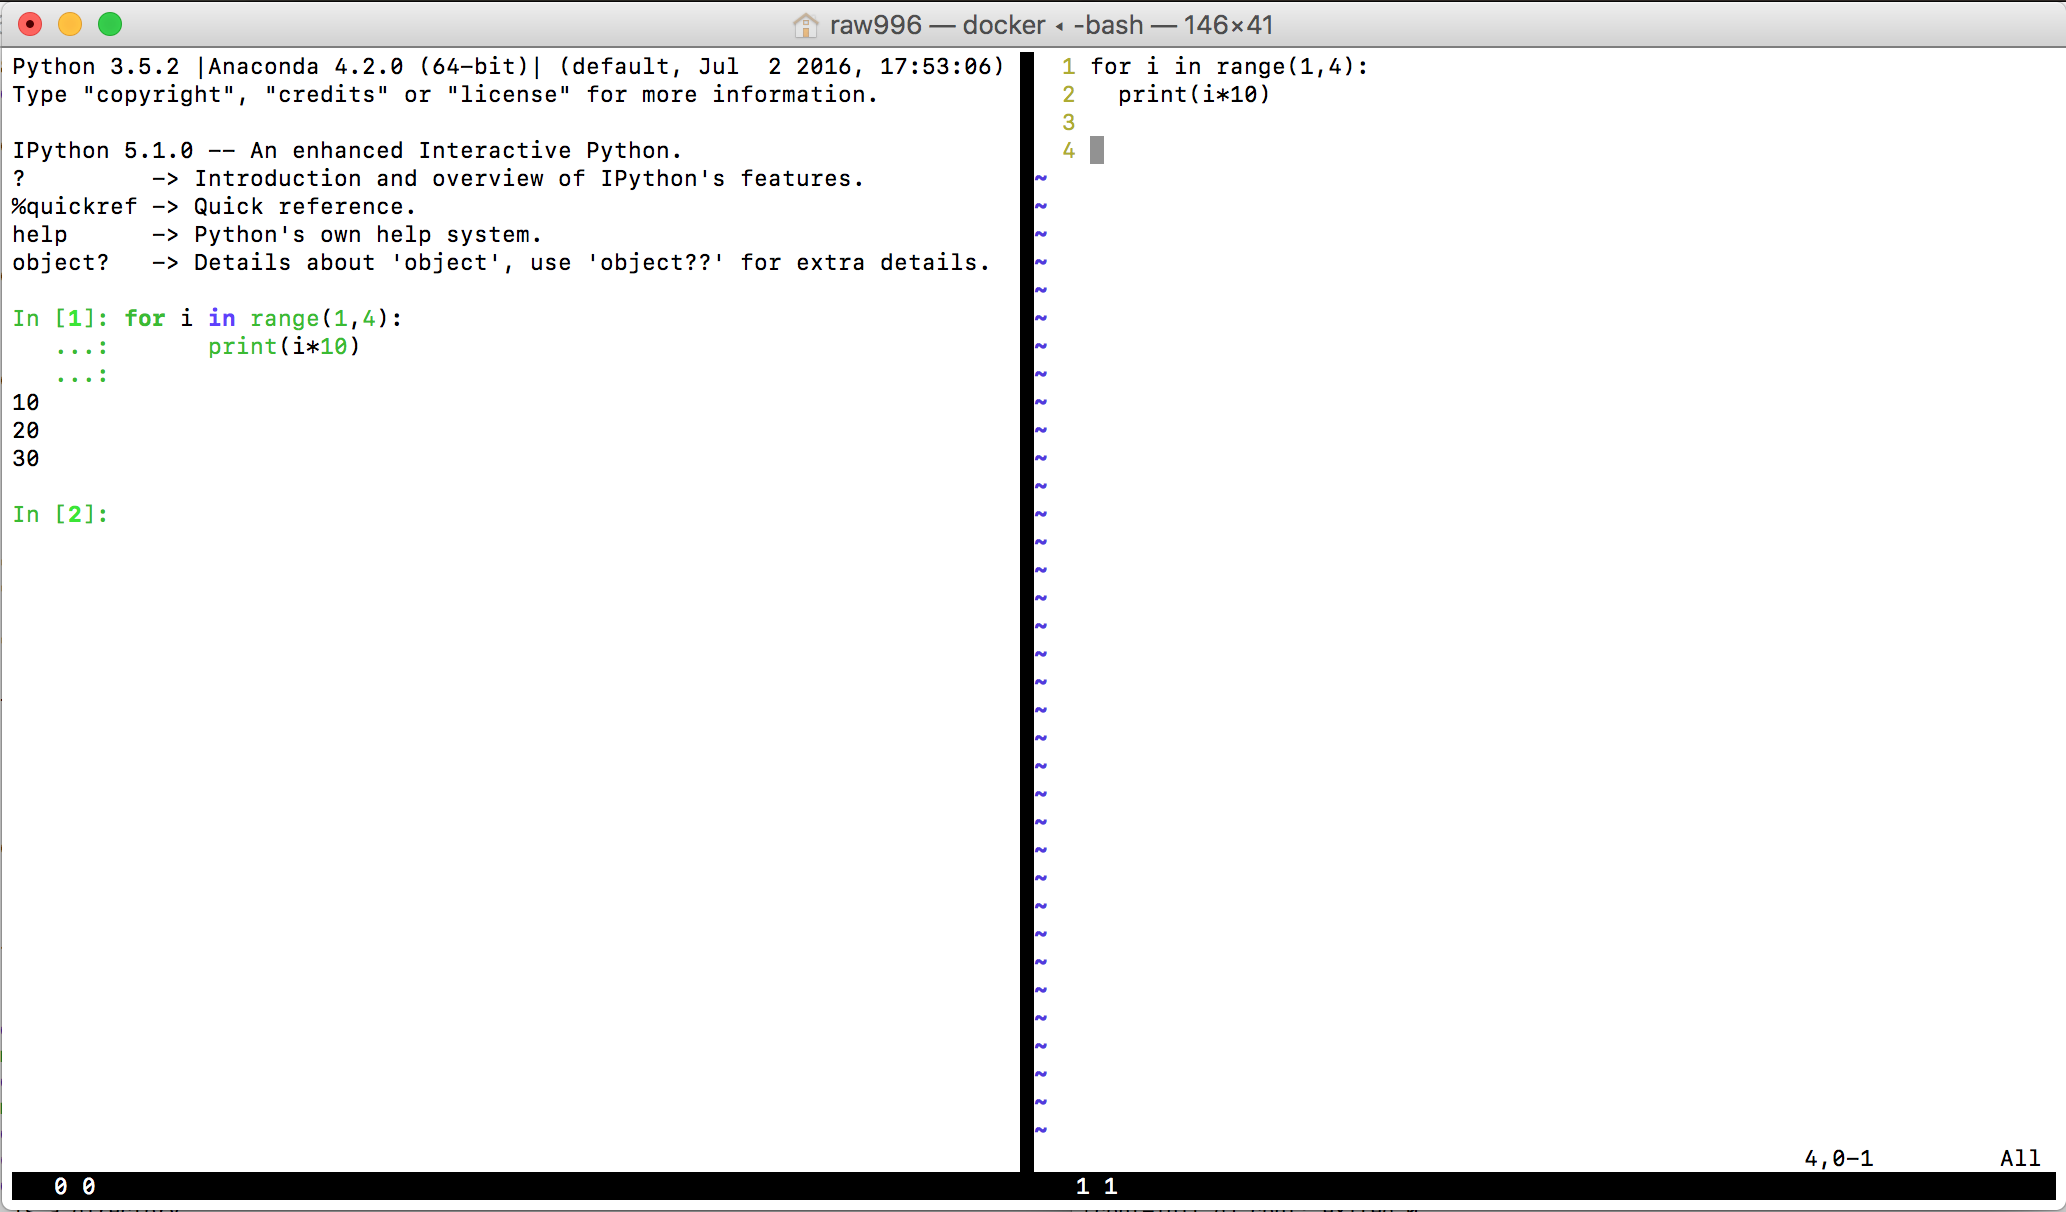
\includegraphics{vim-python.png}
\caption{img}
\end{figure}

\url{https://github.com/jpalardy/vim-slime}

\section{Which Docker containers should I
use?}\label{which-docker-containers-should-i-use}

\url{https://github.com/rocker-org}

\url{https://github.com/Kaggle/docker-python}

\section{Putting it all together}\label{putting-it-all-together}

\url{https://github.com/raubreywhite/docker}

\chapter{Linear Regression vs ANOVA}\label{linear-regression-vs-anova}

\section{Summary}\label{summary}

Many ANOVA computations can be performed using linear regression models,
with nested/hierarchical problems requiring mixed effects regression
models \citep{gelman_analysis_2005}.

\section{Empirical evidence}\label{empirical-evidence}

First we create some data, shown in Figure \ref{fig:anova-data}

\begin{Shaded}
\begin{Highlighting}[]
\KeywordTok{library}\NormalTok{(ggplot2)}

\KeywordTok{set.seed}\NormalTok{(}\DecValTok{4}\NormalTok{)}
\NormalTok{x <-}\StringTok{ }\KeywordTok{rep}\NormalTok{(}\DecValTok{0}\NormalTok{:}\DecValTok{2}\NormalTok{,}\DecValTok{100}\NormalTok{)}
\NormalTok{y <-}\StringTok{ }\NormalTok{(x}\DecValTok{+1}\NormalTok{)/}\DecValTok{7} \NormalTok{+}\StringTok{ }\KeywordTok{rnorm}\NormalTok{(}\KeywordTok{length}\NormalTok{(x))}
\NormalTok{data <-}\StringTok{ }\KeywordTok{data.frame}\NormalTok{(}\DataTypeTok{y=}\NormalTok{y,}\DataTypeTok{x=}\NormalTok{x)}

\NormalTok{q <-}\StringTok{ }\KeywordTok{ggplot}\NormalTok{(data,}\KeywordTok{aes}\NormalTok{(}\DataTypeTok{x=}\NormalTok{x,}\DataTypeTok{y=}\NormalTok{y,}\DataTypeTok{group=}\NormalTok{x))}
\NormalTok{q <-}\StringTok{ }\NormalTok{q +}\StringTok{ }\KeywordTok{geom_boxplot}\NormalTok{()}
\KeywordTok{print}\NormalTok{(q)}
\end{Highlighting}
\end{Shaded}

\begin{figure}

{\centering 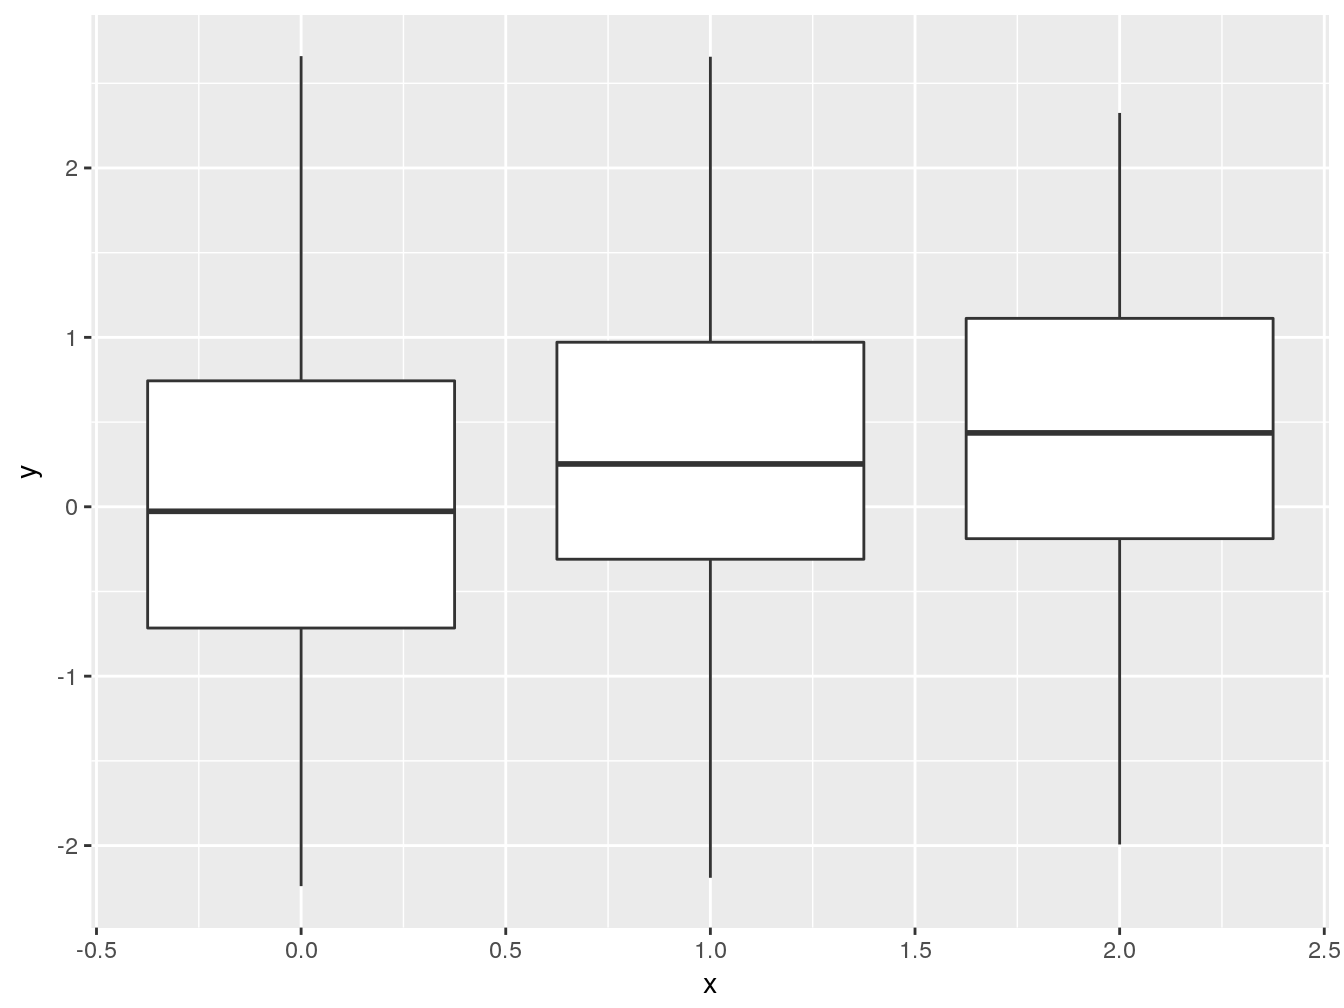
\includegraphics[width=0.8\linewidth]{a-compendium-of-statistics-questions_files/figure-latex/anova-data-1} 

}

\caption{Three diffferent groups (x=0, 1, 2)}\label{fig:anova-data}
\end{figure}

Then we establish the linear regression model

\[
y_i = \beta_0 + \beta_1 x_{1i} + \beta_2 x_{2i} + \epsilon_i
\] where \(i=1,\dots\,n\) and \(\epsilon_i \sim N(0,\sigma^2)\)

\begin{Shaded}
\begin{Highlighting}[]
\NormalTok{fit <-}\StringTok{ }\KeywordTok{lm}\NormalTok{(y ~}\StringTok{ }\KeywordTok{factor}\NormalTok{(x), data)}
\KeywordTok{summary}\NormalTok{(fit)}
\end{Highlighting}
\end{Shaded}

\begin{verbatim}
## 
## Call:
## lm(formula = y ~ factor(x), data = data)
## 
## Residuals:
##      Min       1Q   Median       3Q      Max 
## -2.48573 -0.70825 -0.05413  0.67424  2.59549 
## 
## Coefficients:
##             Estimate Std. Error t value Pr(>|t|)   
## (Intercept)  0.06488    0.09662   0.672  0.50239   
## factor(x)1   0.23052    0.13664   1.687  0.09264 . 
## factor(x)2   0.40818    0.13664   2.987  0.00305 **
## ---
## Signif. codes:  0 '***' 0.001 '**' 0.01 '*' 0.05 '.' 0.1 ' ' 1
## 
## Residual standard error: 0.9662 on 297 degrees of freedom
## Multiple R-squared:  0.02933,    Adjusted R-squared:  0.02279 
## F-statistic: 4.487 on 2 and 297 DF,  p-value: 0.01203
\end{verbatim}

and we can see that the F-test corresponding to

\[
H_0: \beta_1 = \beta_2 = 0
\] \[
H_1: \text{Not } H_0
\] has a p-value of 0.01203.

We then perform a one-way ANOVA assuming equal variances, with: \[
H_0: \bar{y}_{\text{x=0}} = \bar{y}_{\text{x=1}} = \bar{y}_{\text{x=2}}
\] \[
H_1: \text{Not } H_0
\]

\begin{Shaded}
\begin{Highlighting}[]
\KeywordTok{oneway.test}\NormalTok{(y~x,}\DataTypeTok{data =} \NormalTok{data,}\DataTypeTok{var.equal =} \OtherTok{TRUE}\NormalTok{)}
\end{Highlighting}
\end{Shaded}

\begin{verbatim}
## 
##  One-way analysis of means
## 
## data:  y and x
## F = 4.4869, num df = 2, denom df = 297, p-value = 0.01203
\end{verbatim}

and we again see that the p-value is 0.01203.

However, when running a one-way ANOVA assuming unequal variances

\begin{Shaded}
\begin{Highlighting}[]
\KeywordTok{oneway.test}\NormalTok{(y~x,}\DataTypeTok{data =} \NormalTok{data,}\DataTypeTok{var.equal =} \OtherTok{FALSE}\NormalTok{)}
\end{Highlighting}
\end{Shaded}

\begin{verbatim}
## 
##  One-way analysis of means (not assuming equal variances)
## 
## data:  y and x
## F = 4.5345, num df = 2.00, denom df = 197.56, p-value = 0.01187
\end{verbatim}

We see that the p-value is 0.01187, which is not the same as the linear
regression.

\section{Statistical proof}\label{statistical-proof}

The following proof was taken from \citep{hardy_difference_2012}

Suppose your data set consists of a set \((x_i,y_i)\) for
\(i=1,\ldots,n\) and you want to look at the dependence of \(y\) on
\(x\).

Suppose you find the values \(\hat\beta_0\) and \(\hat\beta_1\) of
\(\beta_0\) and \(\beta_1\) that minimize the residual sum of squares \[
\sum_{i=1}^n (y_i - (\beta_0+\beta_1 x_i))^2.
\] Then you take \(\hat y = \hat\beta_0+ \hat\beta_1 x\) to be the
predicted \(y\)-value for any (not necessarily already observed)
\(x\)-value. That's linear regression.

Now consider decomposing the total sum of squares \[
\sum_{i=1}^n (y_i - \bar y)^2 \text{ where }\bar y = \frac{y_1+\cdots+y_n}{n}
\] with \(n-1\) degrees of freedom, into ``explained'' and
``unexplained'' parts: \[
\underbrace{\sum_{i=1}^n ((\hat\beta_0+\hat\beta_1 x_i) - \bar y)^2}_{\text{explained}}\  +\  \underbrace{\sum_{i=1}^n (y_i - (\hat\beta_0+\hat\beta_1 x_i))^2}_{\text{unexplained}}.
\] with \(1\) and \(n-2\) degrees of freedom, respectively. That's
analysis of variance, and one then considers things like F-statistics \[
F = \frac{\sum_{i=1}^n ((\hat\beta_0+\hat\beta_1 x_i) - \bar y)^2/1}{\sum_{i=1}^n (y_i - (\hat\beta_0+\hat\beta_1 x_i))^2/(n-2)}.
\] \emph{This} F-statistic tests the null hypothesis \(\beta_1=0\),
which is the same as the traditional ANOVA: \[
F = \frac{\text{Between SS}/\text{df}}{\text{Within SS}/\text{df}}.
\]

One often first encounters the term ``analysis of variance'' when the
predictor is categorical, so that you're fitting the model \[
y = \beta_0 + \beta_i
\] where \(i\) identifies which category is the value of the predictor.
If there are \(k\) categories, you'd get \(k-1\) degrees of freedom in
the numerator in the F-statistic, and usually \(n-k\) degrees of freedom
in the denominator. But the distinction between regression and analysis
of variance is still the same for this kind of model.

\chapter{Outcomes}\label{outcomes}

\section{Length of stay}\label{length-of-stay}

If your outcome is length of stay in a hospital, you should consider
using a generalized linear model with Poisson or negative binomial
distribution or Gaussian with log link \citep{austin_comparison_2002}.

\chapter{Multiple imputation}\label{multiple-imputation}

\section{Longitudinal data}\label{longitudinal-data}

If the longitudinal measurements were taken at roughly ordered intervals
(e.g. ``1 month checkup'', ``5 month checkup''), then try to reshape the
data to wide format (one row per person) and then perform multiple
imputations
\citep[\citet{statistical_consulting_group_ucla_how_2017}]{allison_missing_2002}.

\chapter{Regressions using survey
data}\label{regressions-using-survey-data}

\section{Literature summary}\label{literature-summary}

\begin{itemize}
\tightlist
\item
  Endogenous sampling can be thought of as cases where the regression
  error term is related to the sampling criteria
  \citep[\citet{solon_what_2013},
  \citet{fuller_sampling_2009}]{friedman_tools_2013}
\item
  In the presence of endogenous sampling, unweighted estimates may be
  biased, but will be corrected by weighting by the inverse probability
  of selection \citep[\citet{solon_what_2013},
  \citet{fuller_sampling_2009}]{friedman_tools_2013}
\item
  In the presence of endogenous sampling, if the sampling probability
  varies across certain strata and those strata indicators are included
  in the estimating equation, then the probability of selection should
  no longer be related to the error term. Subsequently, weighting is not
  necessary \citep[\citet{solon_what_2013},
  \citet{fuller_sampling_2009}]{friedman_tools_2013}
\item
  In the case of a linear regression model that correctly specifies the
  conditional mean, the sampling would be exogenous if the sampling
  probabilities are independent of the error term in the regression
  equation. This would be the case, for example, if the sampling
  probabilities vary only on the basis of explanatory variables
  \citep{solon_what_2013}
\item
  More generally, the issue is whether the sampling is independent of
  the dependent variable conditional on the explanatory variables
  \citep{solon_what_2013}
\item
  Weighting does not correct for confounding. Adjusting for confounders
  is still necessary.
\item
  Weighting is useful when the regression model that accounts for
  sampling probabilities does not make any sense (e.g.~in the
  case-control scenario).
\end{itemize}

\section{Setup}\label{setup}

\begin{Shaded}
\begin{Highlighting}[]
\NormalTok{FormatNicely <-}\StringTok{ }\NormalTok{function(x,}\DataTypeTok{dp=}\DecValTok{3}\NormalTok{)\{}
  \KeywordTok{formatC}\NormalTok{(x,}\DataTypeTok{digits=}\NormalTok{dp,}\DataTypeTok{format=}\StringTok{"f"}\NormalTok{)}
\NormalTok{\}}

\NormalTok{ConvertFitToResults <-}\StringTok{ }\NormalTok{function(fit,dataName,analysisName)\{}
  \NormalTok{r <-}\StringTok{ }\KeywordTok{data.frame}\NormalTok{(}\KeywordTok{coef}\NormalTok{(}\KeywordTok{summary}\NormalTok{(fit)))[-}\DecValTok{1}\NormalTok{,-}\KeywordTok{c}\NormalTok{(}\DecValTok{3}\NormalTok{:}\DecValTok{4}\NormalTok{),drop=F]}
  \NormalTok{r[,}\DecValTok{1}\NormalTok{] <-}\StringTok{ }\KeywordTok{sprintf}\NormalTok{(}\StringTok{"%s [%s]"}\NormalTok{,}
                   \KeywordTok{FormatNicely}\NormalTok{(r[,}\DecValTok{1}\NormalTok{],}\DataTypeTok{dp=}\DecValTok{3}\NormalTok{),}
                   \KeywordTok{FormatNicely}\NormalTok{(r[,}\DecValTok{2}\NormalTok{],}\DataTypeTok{dp=}\DecValTok{3}\NormalTok{))}
  \NormalTok{r <-}\StringTok{ }\NormalTok{r[,}\DecValTok{1}\NormalTok{,drop=F]}
  \NormalTok{r <-}\StringTok{ }\KeywordTok{as.data.frame}\NormalTok{(}\KeywordTok{t}\NormalTok{(r))}
  \NormalTok{r$data <-}\StringTok{ }\NormalTok{dataName}
  \NormalTok{r$analysis <-}\StringTok{ }\NormalTok{analysisName}
  \KeywordTok{return}\NormalTok{(r)}
\NormalTok{\}}
\end{Highlighting}
\end{Shaded}

\section{Case-control studies}\label{case-control-studies}

In this case study we will create a dataset \texttt{popData} that has a
1:1 linear relationship between the continuous exposure \texttt{x} and
and the continuous outcome \texttt{y}. We also dichotomise \texttt{y}
into a binary outcome \texttt{yBinary}.

We then create a dataset \texttt{casecontrolData} that oversamples cases
5x higher than is found in the normal population \texttt{popData}. We
will then run linear regressions in the original population dataset and
the case-control dataset and see how the effect estimates are affected
by oversampling cases.

\begin{Shaded}
\begin{Highlighting}[]
\KeywordTok{library}\NormalTok{(data.table)}

\CommentTok{# Creating population dataset}
\NormalTok{x <-}\StringTok{ }\KeywordTok{runif}\NormalTok{(}\DecValTok{100000}\NormalTok{)}
\NormalTok{popData <-}\StringTok{ }\KeywordTok{data.table}\NormalTok{(x)}
\NormalTok{popData[,y:}\ErrorTok{=}\NormalTok{x+}\KeywordTok{rnorm}\NormalTok{(.N)]}

\CommentTok{# Binary outcome}
\NormalTok{popData[,yBinary:}\ErrorTok{=}\DecValTok{0}\NormalTok{]}
\NormalTok{popData[y>}\DecValTok{1}\NormalTok{,yBinary:}\ErrorTok{=}\DecValTok{1}\NormalTok{]}
\NormalTok{popData[,oversampled:}\ErrorTok{=}\NormalTok{yBinary]}

\NormalTok{popData[,inclusionProb :}\ErrorTok{=}\StringTok{ }\DecValTok{5}\NormalTok{]}
\NormalTok{popData[oversampled==}\DecValTok{0}\NormalTok{, inclusionProb:}\ErrorTok{=}\DecValTok{1}\NormalTok{]}

\CommentTok{# Case control dataset}
\NormalTok{cases <-}\StringTok{ }\NormalTok{popData[yBinary==}\DecValTok{1}\NormalTok{]}
\NormalTok{controls <-}\StringTok{ }\NormalTok{popData[yBinary==}\DecValTok{0}\NormalTok{]}

\CommentTok{# Cases are sampled 5x higher than normal}
\NormalTok{casecontrolData <-}\StringTok{ }\KeywordTok{rbind}\NormalTok{(cases,cases,cases,cases,cases,controls)}
\NormalTok{casecontrolData[,id:}\ErrorTok{=}\DecValTok{1}\NormalTok{:.N]}
\end{Highlighting}
\end{Shaded}

\begin{Shaded}
\begin{Highlighting}[]
\CommentTok{# Full population data set, unweighted regression}
\NormalTok{res <-}\StringTok{ }\KeywordTok{vector}\NormalTok{(}\StringTok{"list"}\NormalTok{,}\DecValTok{10}\NormalTok{)}
\NormalTok{fit <-}\StringTok{ }\KeywordTok{glm}\NormalTok{(y~x,}\DataTypeTok{data=}\NormalTok{popData)}
\NormalTok{res[[}\DecValTok{1}\NormalTok{]] <-}\StringTok{ }\KeywordTok{ConvertFitToResults}\NormalTok{(fit,}\DataTypeTok{dataName=}\StringTok{"Pop"}\NormalTok{,}\DataTypeTok{analysisName=}\StringTok{"Unweighted"}\NormalTok{)}
\NormalTok{res[[}\DecValTok{1}\NormalTok{]]$correlation <-}\StringTok{ }\KeywordTok{FormatNicely}\NormalTok{(}\KeywordTok{cor}\NormalTok{(}\KeywordTok{resid}\NormalTok{(fit),fit$data$oversampled), }\DataTypeTok{dp=}\DecValTok{2}\NormalTok{)}

\CommentTok{# Biased dataset (case control with 5x), unweighted regression}
\NormalTok{fit <-}\StringTok{ }\KeywordTok{glm}\NormalTok{(y~x,}\DataTypeTok{data=}\NormalTok{casecontrolData)}
\NormalTok{res[[}\DecValTok{2}\NormalTok{]] <-}\StringTok{ }\KeywordTok{ConvertFitToResults}\NormalTok{(fit,}\DataTypeTok{dataName=}\StringTok{"Sample"}\NormalTok{,}\DataTypeTok{analysisName=}\StringTok{"Unweighted"}\NormalTok{)}
\NormalTok{res[[}\DecValTok{2}\NormalTok{]]$correlation <-}\StringTok{ }\KeywordTok{FormatNicely}\NormalTok{(}\KeywordTok{cor}\NormalTok{(}\KeywordTok{resid}\NormalTok{(fit),fit$data$oversampled), }\DataTypeTok{dp=}\DecValTok{2}\NormalTok{)}

\CommentTok{# Biased dataset (case control with 5x), weighted regression}
\NormalTok{des <-}\StringTok{ }\NormalTok{survey::}\KeywordTok{svydesign}\NormalTok{(}\DataTypeTok{id=}\NormalTok{~id,}\DataTypeTok{prob=}\NormalTok{~inclusionProb,}\DataTypeTok{data=}\NormalTok{casecontrolData)}
\NormalTok{fit <-}\StringTok{ }\NormalTok{survey::}\KeywordTok{svyglm}\NormalTok{(y~x, }\DataTypeTok{design=}\NormalTok{des)}
\NormalTok{res[[}\DecValTok{3}\NormalTok{]] <-}\StringTok{ }\KeywordTok{ConvertFitToResults}\NormalTok{(fit,}\DataTypeTok{dataName=}\StringTok{"Sample"}\NormalTok{,}\DataTypeTok{analysisName=}\StringTok{"Weighted"}\NormalTok{)}
\NormalTok{res[[}\DecValTok{3}\NormalTok{]]$correlation <-}\StringTok{ }\KeywordTok{FormatNicely}\NormalTok{(}\KeywordTok{cor}\NormalTok{(}\KeywordTok{resid}\NormalTok{(fit),fit$data$oversampled), }\DataTypeTok{dp=}\DecValTok{2}\NormalTok{)}

\NormalTok{res <-}\StringTok{ }\KeywordTok{rbindlist}\NormalTok{(res,}\DataTypeTok{fill=}\NormalTok{T)}
\KeywordTok{setcolorder}\NormalTok{(res, }\KeywordTok{c}\NormalTok{(}\StringTok{"data"}\NormalTok{, }\StringTok{"analysis"}\NormalTok{, }\StringTok{"x"}\NormalTok{, }\StringTok{"correlation"}\NormalTok{))}
\KeywordTok{setnames}\NormalTok{(res, }\KeywordTok{c}\NormalTok{(}\StringTok{"Data"}\NormalTok{, }\StringTok{"Analysis"}\NormalTok{, }\StringTok{"coef(x) [sd(coef(x))]"}\NormalTok{, }\StringTok{"Correlation*"}\NormalTok{))}

\NormalTok{knitr::}\KeywordTok{kable}\NormalTok{(}
  \NormalTok{res, }\DataTypeTok{booktabs =} \OtherTok{TRUE}\NormalTok{,}
  \DataTypeTok{caption =} \StringTok{'Effects of weights on linear regression coefficient estimates. (*Correlation between residuals and sampling probability).'}
\NormalTok{)}
\end{Highlighting}
\end{Shaded}

\begin{table}

\caption{\label{tab:unnamed-chunk-5}Effects of weights on linear regression coefficient estimates. (*Correlation between residuals and sampling probability).}
\centering
\begin{tabular}[t]{llll}
\toprule
Data & Analysis & coef(x) [sd(coef(x))] & Correlation*\\
\midrule
Pop & Unweighted & 0.989 [0.011] & 0.74\\
Sample & Unweighted & 0.910 [0.007] & 0.77\\
Sample & Weighted & 0.989 [0.009] & 0.71\\
\bottomrule
\end{tabular}
\end{table}

We can see here that in the presence of endogenous sampling, the
sampling probability is highly correlated with the regression error
term. By weighting the data by the inverse probability of selection we
obtain unbiased estimates of \texttt{coef(x)}.

\section{Oversampling a population with a higher level of the
outcome}\label{oversampling-a-population-with-a-higher-level-of-the-outcome}

\begin{Shaded}
\begin{Highlighting}[]
\KeywordTok{library}\NormalTok{(data.table)}

\CommentTok{# Creating population dataset}
\NormalTok{x <-}\StringTok{ }\KeywordTok{runif}\NormalTok{(}\DecValTok{100000}\NormalTok{)}
\NormalTok{popData <-}\StringTok{ }\KeywordTok{data.table}\NormalTok{(x)}
\NormalTok{popData[,poor:}\ErrorTok{=}\DecValTok{0}\NormalTok{]}
\NormalTok{popData[}\DecValTok{1}\NormalTok{:}\DecValTok{10000}\NormalTok{,poor:}\ErrorTok{=}\DecValTok{1}\NormalTok{]}
\NormalTok{popData[,bmi:}\ErrorTok{=}\DecValTok{22+1}\NormalTok{*x}\DecValTok{+5}\NormalTok{*poor+}\KeywordTok{rnorm}\NormalTok{(.N)*}\DecValTok{2}\NormalTok{]}

\CommentTok{# Oversampled poor dataset}
\NormalTok{poor <-}\StringTok{ }\NormalTok{popData[poor==}\DecValTok{1}\NormalTok{]}
\NormalTok{notpoor <-}\StringTok{ }\NormalTok{popData[poor==}\DecValTok{0}\NormalTok{]}

\CommentTok{# Poor people are sampled 5x higher than not-poor}
\NormalTok{oversampledData <-}\StringTok{ }\KeywordTok{rbind}\NormalTok{(poor,poor,poor,poor,poor,notpoor)}
\NormalTok{oversampledData[,id:}\ErrorTok{=}\DecValTok{1}\NormalTok{:.N]}

\CommentTok{# Probability of inclusion}
\NormalTok{oversampledData[,inclusionProb :}\ErrorTok{=}\StringTok{ }\DecValTok{5}\NormalTok{]}
\NormalTok{oversampledData[poor==}\DecValTok{0}\NormalTok{, inclusionProb:}\ErrorTok{=}\DecValTok{1}\NormalTok{]}
\end{Highlighting}
\end{Shaded}

\begin{Shaded}
\begin{Highlighting}[]
\CommentTok{# Full population data set, unweighted regression}
\NormalTok{res <-}\StringTok{ }\KeywordTok{vector}\NormalTok{(}\StringTok{"list"}\NormalTok{,}\DecValTok{10}\NormalTok{)}
\NormalTok{res[[}\DecValTok{1}\NormalTok{]] <-}\StringTok{ }\KeywordTok{ConvertFitToResults}\NormalTok{(fit <-}\StringTok{ }\KeywordTok{glm}\NormalTok{(bmi~x,}\DataTypeTok{data=}\NormalTok{popData),}
                                \DataTypeTok{dataName=}\StringTok{"Pop"}\NormalTok{,}\DataTypeTok{analysisName=}\StringTok{"Unweighted"}\NormalTok{)}
\NormalTok{res[[}\DecValTok{1}\NormalTok{]]$correlation <-}\StringTok{ }\KeywordTok{FormatNicely}\NormalTok{(}\KeywordTok{cor}\NormalTok{(}\KeywordTok{resid}\NormalTok{(fit),fit$data$poor), }\DataTypeTok{dp=}\DecValTok{2}\NormalTok{)}

\CommentTok{# Biased dataset (poor oversampled 5x), unweighted regression}
\NormalTok{res[[}\DecValTok{2}\NormalTok{]] <-}\StringTok{ }\KeywordTok{ConvertFitToResults}\NormalTok{(fit <-}\StringTok{ }\KeywordTok{glm}\NormalTok{(bmi~x,}\DataTypeTok{data=}\NormalTok{oversampledData),}
                                \DataTypeTok{dataName=}\StringTok{"Sample"}\NormalTok{,}\DataTypeTok{analysisName=}\StringTok{"Unweighted"}\NormalTok{)}
\NormalTok{res[[}\DecValTok{2}\NormalTok{]]$correlation <-}\StringTok{ }\KeywordTok{FormatNicely}\NormalTok{(}\KeywordTok{cor}\NormalTok{(}\KeywordTok{resid}\NormalTok{(fit),fit$data$poor), }\DataTypeTok{dp=}\DecValTok{2}\NormalTok{)}

\CommentTok{# Biased dataset (poor oversampled 5x), weighted regression}
\NormalTok{des <-}\StringTok{ }\NormalTok{survey::}\KeywordTok{svydesign}\NormalTok{(}\DataTypeTok{id=}\NormalTok{~id,}\DataTypeTok{prob=}\NormalTok{~inclusionProb,}\DataTypeTok{data=}\NormalTok{oversampledData)}
\NormalTok{res[[}\DecValTok{3}\NormalTok{]] <-}\StringTok{ }\KeywordTok{ConvertFitToResults}\NormalTok{(fit <-}\StringTok{ }\NormalTok{survey::}\KeywordTok{svyglm}\NormalTok{(bmi~x, }\DataTypeTok{design=}\NormalTok{des),}
                                \DataTypeTok{dataName=}\StringTok{"Sample"}\NormalTok{,}\DataTypeTok{analysisName=}\StringTok{"Weighted"}\NormalTok{)}
\NormalTok{res[[}\DecValTok{3}\NormalTok{]]$correlation <-}\StringTok{ }\KeywordTok{FormatNicely}\NormalTok{(}\KeywordTok{cor}\NormalTok{(}\KeywordTok{resid}\NormalTok{(fit),fit$data$poor), }\DataTypeTok{dp=}\DecValTok{2}\NormalTok{)}

\CommentTok{# Full population data set, unweighted regression + strata indicator}
\NormalTok{res[[}\DecValTok{4}\NormalTok{]] <-}\StringTok{ }\KeywordTok{ConvertFitToResults}\NormalTok{(fit <-}\StringTok{ }\KeywordTok{glm}\NormalTok{(bmi~x+poor,}\DataTypeTok{data=}\NormalTok{popData),}
                                \DataTypeTok{dataName=}\StringTok{"Pop"}\NormalTok{,}\DataTypeTok{analysisName=}\StringTok{"Unweighted+Strata"}\NormalTok{)}
\NormalTok{res[[}\DecValTok{4}\NormalTok{]]$correlation <-}\StringTok{ }\KeywordTok{FormatNicely}\NormalTok{(}\KeywordTok{cor}\NormalTok{(}\KeywordTok{resid}\NormalTok{(fit),fit$data$poor), }\DataTypeTok{dp=}\DecValTok{2}\NormalTok{)}

\CommentTok{# Biased dataset (poor oversampled 5x), unweighted regression + strata indicator}
\NormalTok{res[[}\DecValTok{5}\NormalTok{]] <-}\StringTok{ }\KeywordTok{ConvertFitToResults}\NormalTok{(fit <-}\StringTok{ }\KeywordTok{glm}\NormalTok{(bmi~x+poor,}\DataTypeTok{data=}\NormalTok{oversampledData),}
                                \DataTypeTok{dataName=}\StringTok{"Sample"}\NormalTok{,}\DataTypeTok{analysisName=}\StringTok{"Unweighted+Strata"}\NormalTok{)}
\NormalTok{res[[}\DecValTok{5}\NormalTok{]]$correlation <-}\StringTok{ }\KeywordTok{FormatNicely}\NormalTok{(}\KeywordTok{cor}\NormalTok{(}\KeywordTok{resid}\NormalTok{(fit),fit$data$poor), }\DataTypeTok{dp=}\DecValTok{2}\NormalTok{)}

\CommentTok{# Biased dataset (poor oversampled 5x), weighted regression + strata indicator}
\NormalTok{des <-}\StringTok{ }\NormalTok{survey::}\KeywordTok{svydesign}\NormalTok{(}\DataTypeTok{id=}\NormalTok{~id,}\DataTypeTok{prob=}\NormalTok{~inclusionProb,}\DataTypeTok{data=}\NormalTok{oversampledData)}
\NormalTok{res[[}\DecValTok{6}\NormalTok{]] <-}\StringTok{ }\KeywordTok{ConvertFitToResults}\NormalTok{(fit <-}\StringTok{ }\NormalTok{survey::}\KeywordTok{svyglm}\NormalTok{(bmi~x+poor, }\DataTypeTok{design=}\NormalTok{des),}
                                \DataTypeTok{dataName=}\StringTok{"Sample"}\NormalTok{,}\DataTypeTok{analysisName=}\StringTok{"Weighted+Strata"}\NormalTok{)}
\NormalTok{res[[}\DecValTok{6}\NormalTok{]]$correlation <-}\StringTok{ }\KeywordTok{FormatNicely}\NormalTok{(}\KeywordTok{cor}\NormalTok{(}\KeywordTok{resid}\NormalTok{(fit),fit$data$poor), }\DataTypeTok{dp=}\DecValTok{2}\NormalTok{)}

\NormalTok{res <-}\StringTok{ }\KeywordTok{rbindlist}\NormalTok{(res,}\DataTypeTok{fill=}\NormalTok{T)}
\KeywordTok{setcolorder}\NormalTok{(res,}\KeywordTok{c}\NormalTok{(}\StringTok{"data"}\NormalTok{, }\StringTok{"analysis"}\NormalTok{, }\StringTok{"x"}\NormalTok{, }\StringTok{"poor"}\NormalTok{, }\StringTok{"correlation"}\NormalTok{))}
\KeywordTok{setnames}\NormalTok{(res,}\KeywordTok{c}\NormalTok{(}\StringTok{"Data"}\NormalTok{, }\StringTok{"Analysis"}\NormalTok{, }\StringTok{"coef(x) [sd(coef(x))]"}\NormalTok{, }\StringTok{"coef(poor) [sd(coef(poor))]"}\NormalTok{, }\StringTok{"Correlation*"}\NormalTok{))}

\NormalTok{knitr::}\KeywordTok{kable}\NormalTok{(}
  \NormalTok{res, }\DataTypeTok{booktabs =} \OtherTok{TRUE}\NormalTok{,}
  \DataTypeTok{caption =} \StringTok{'Effects of weights on linear regression coefficient estimates. (*Correlation between residuals and sampling probability).'}
\NormalTok{)}
\end{Highlighting}
\end{Shaded}

\begin{table}

\caption{\label{tab:unnamed-chunk-7}Effects of weights on linear regression coefficient estimates. (*Correlation between residuals and sampling probability).}
\centering
\begin{tabular}[t]{lllll}
\toprule
Data & Analysis & coef(x) [sd(coef(x))] & coef(poor) [sd(coef(poor))] & Correlation*\\
\midrule
Pop & Unweighted & 1.060 [0.027] & NA & 0.60\\
Sample & Unweighted & 1.108 [0.029] & NA & 0.77\\
Sample & Weighted & 1.060 [0.023] & NA & 0.58\\
Pop & Unweighted+Strata & 1.032 [0.022] & 5.012 [0.021] & 0.00\\
Sample & Unweighted+Strata & 1.036 [0.018] & 5.012 [0.011] & 0.00\\
Sample & Weighted+Strata & 1.032 [0.021] & 5.012 [0.011] & 0.00\\
\bottomrule
\end{tabular}
\end{table}

We can see here that in the first three models the sampling probability
is highly correlated with the regression error term. Models 1 and 3
provide unbiased estimates (through exogenous sampling and weighting,
respectively.) In models 4 through to 6, we included an explanatory
variable \texttt{poor} to account for the varying sampling
probabilities. Subsequently, the sampling probability is no longer
correlated with the regression error term, and we obtain unbiased
estimates.

\section{Oversampling a population with a higher level of the outcome
and
exposure}\label{oversampling-a-population-with-a-higher-level-of-the-outcome-and-exposure}

\begin{Shaded}
\begin{Highlighting}[]
\KeywordTok{library}\NormalTok{(data.table)}

\CommentTok{# Creating population dataset}
\NormalTok{x <-}\StringTok{ }\KeywordTok{runif}\NormalTok{(}\DecValTok{100000}\NormalTok{)}
\NormalTok{popData <-}\StringTok{ }\KeywordTok{data.table}\NormalTok{(x)}
\NormalTok{popData[,poor:}\ErrorTok{=}\DecValTok{0}\NormalTok{]}
\NormalTok{popData[}\DecValTok{1}\NormalTok{:}\DecValTok{10000}\NormalTok{,poor:}\ErrorTok{=}\DecValTok{1}\NormalTok{]}
\NormalTok{popData[,x:}\ErrorTok{=}\NormalTok{x}\DecValTok{+2}\NormalTok{*poor]}
\NormalTok{popData[,bmi:}\ErrorTok{=}\DecValTok{22+1}\NormalTok{*x}\DecValTok{+5}\NormalTok{*poor+}\KeywordTok{rnorm}\NormalTok{(.N)*}\DecValTok{2}\NormalTok{]}

\CommentTok{# Oversampled poor dataset}
\NormalTok{poor <-}\StringTok{ }\NormalTok{popData[poor==}\DecValTok{1}\NormalTok{]}
\NormalTok{notpoor <-}\StringTok{ }\NormalTok{popData[poor==}\DecValTok{0}\NormalTok{]}

\CommentTok{# Poor people are sampled 5x higher than not-poor}
\NormalTok{oversampledData <-}\StringTok{ }\KeywordTok{rbind}\NormalTok{(poor,poor,poor,poor,poor,notpoor)}
\NormalTok{oversampledData[,id:}\ErrorTok{=}\DecValTok{1}\NormalTok{:.N]}

\CommentTok{# Probability of inclusion}
\NormalTok{oversampledData[,inclusionProb :}\ErrorTok{=}\StringTok{ }\DecValTok{5}\NormalTok{]}
\NormalTok{oversampledData[poor==}\DecValTok{0}\NormalTok{, inclusionProb:}\ErrorTok{=}\DecValTok{1}\NormalTok{]}
\end{Highlighting}
\end{Shaded}

\begin{Shaded}
\begin{Highlighting}[]
\CommentTok{# Full population data set, unweighted regression}
\NormalTok{res <-}\StringTok{ }\KeywordTok{vector}\NormalTok{(}\StringTok{"list"}\NormalTok{,}\DecValTok{10}\NormalTok{)}
\NormalTok{res[[}\DecValTok{1}\NormalTok{]] <-}\StringTok{ }\KeywordTok{ConvertFitToResults}\NormalTok{(fit <-}\StringTok{ }\KeywordTok{glm}\NormalTok{(bmi~x,}\DataTypeTok{data=}\NormalTok{popData),}
                                \DataTypeTok{dataName=}\StringTok{"Pop"}\NormalTok{,}\DataTypeTok{analysisName=}\StringTok{"Unweighted"}\NormalTok{)}
\NormalTok{res[[}\DecValTok{1}\NormalTok{]]$correlation <-}\StringTok{ }\KeywordTok{FormatNicely}\NormalTok{(}\KeywordTok{cor}\NormalTok{(}\KeywordTok{resid}\NormalTok{(fit),fit$data$poor), }\DataTypeTok{dp=}\DecValTok{2}\NormalTok{)}

\CommentTok{# Biased dataset (poor oversampled 5x), unweighted regression}
\NormalTok{res[[}\DecValTok{2}\NormalTok{]] <-}\StringTok{ }\KeywordTok{ConvertFitToResults}\NormalTok{(fit <-}\StringTok{ }\KeywordTok{glm}\NormalTok{(bmi~x,}\DataTypeTok{data=}\NormalTok{oversampledData),}
                                \DataTypeTok{dataName=}\StringTok{"Sample"}\NormalTok{,}\DataTypeTok{analysisName=}\StringTok{"Unweighted"}\NormalTok{)}
\NormalTok{res[[}\DecValTok{2}\NormalTok{]]$correlation <-}\StringTok{ }\KeywordTok{FormatNicely}\NormalTok{(}\KeywordTok{cor}\NormalTok{(}\KeywordTok{resid}\NormalTok{(fit),fit$data$poor), }\DataTypeTok{dp=}\DecValTok{2}\NormalTok{)}

\CommentTok{# Biased dataset (poor oversampled 5x), weighted regression}
\NormalTok{des <-}\StringTok{ }\NormalTok{survey::}\KeywordTok{svydesign}\NormalTok{(}\DataTypeTok{id=}\NormalTok{~id,}\DataTypeTok{prob=}\NormalTok{~inclusionProb,}\DataTypeTok{data=}\NormalTok{oversampledData)}
\NormalTok{res[[}\DecValTok{3}\NormalTok{]] <-}\StringTok{ }\KeywordTok{ConvertFitToResults}\NormalTok{(fit <-}\StringTok{ }\NormalTok{survey::}\KeywordTok{svyglm}\NormalTok{(bmi~x, }\DataTypeTok{design=}\NormalTok{des),}
                                \DataTypeTok{dataName=}\StringTok{"Sample"}\NormalTok{,}\DataTypeTok{analysisName=}\StringTok{"Weighted"}\NormalTok{)}
\NormalTok{res[[}\DecValTok{3}\NormalTok{]]$correlation <-}\StringTok{ }\KeywordTok{FormatNicely}\NormalTok{(}\KeywordTok{cor}\NormalTok{(}\KeywordTok{resid}\NormalTok{(fit),fit$data$poor), }\DataTypeTok{dp=}\DecValTok{2}\NormalTok{)}

\CommentTok{# Full population data set, unweighted regression + strata indicator}
\NormalTok{res[[}\DecValTok{4}\NormalTok{]] <-}\StringTok{ }\KeywordTok{ConvertFitToResults}\NormalTok{(fit <-}\StringTok{ }\KeywordTok{glm}\NormalTok{(bmi~x+poor,}\DataTypeTok{data=}\NormalTok{popData),}
                                \DataTypeTok{dataName=}\StringTok{"Pop"}\NormalTok{,}\DataTypeTok{analysisName=}\StringTok{"Unweighted+Strata"}\NormalTok{)}
\NormalTok{res[[}\DecValTok{4}\NormalTok{]]$correlation <-}\StringTok{ }\KeywordTok{FormatNicely}\NormalTok{(}\KeywordTok{cor}\NormalTok{(}\KeywordTok{resid}\NormalTok{(fit),fit$data$poor), }\DataTypeTok{dp=}\DecValTok{2}\NormalTok{)}

\CommentTok{# Biased dataset (poor oversampled 5x), unweighted regression + strata indicator}
\NormalTok{res[[}\DecValTok{5}\NormalTok{]] <-}\StringTok{ }\KeywordTok{ConvertFitToResults}\NormalTok{(fit <-}\StringTok{ }\KeywordTok{glm}\NormalTok{(bmi~x+poor,}\DataTypeTok{data=}\NormalTok{oversampledData),}
                                \DataTypeTok{dataName=}\StringTok{"Sample"}\NormalTok{,}\DataTypeTok{analysisName=}\StringTok{"Unweighted+Strata"}\NormalTok{)}
\NormalTok{res[[}\DecValTok{5}\NormalTok{]]$correlation <-}\StringTok{ }\KeywordTok{FormatNicely}\NormalTok{(}\KeywordTok{cor}\NormalTok{(}\KeywordTok{resid}\NormalTok{(fit),fit$data$poor), }\DataTypeTok{dp=}\DecValTok{2}\NormalTok{)}

\CommentTok{# Biased dataset (poor oversampled 5x), weighted regression + strata indicator}
\NormalTok{des <-}\StringTok{ }\NormalTok{survey::}\KeywordTok{svydesign}\NormalTok{(}\DataTypeTok{id=}\NormalTok{~id,}\DataTypeTok{prob=}\NormalTok{~inclusionProb,}\DataTypeTok{data=}\NormalTok{oversampledData)}
\NormalTok{res[[}\DecValTok{6}\NormalTok{]] <-}\StringTok{ }\KeywordTok{ConvertFitToResults}\NormalTok{(fit <-}\StringTok{ }\NormalTok{survey::}\KeywordTok{svyglm}\NormalTok{(bmi~x+poor, }\DataTypeTok{design=}\NormalTok{des),}
                                \DataTypeTok{dataName=}\StringTok{"Sample"}\NormalTok{,}\DataTypeTok{analysisName=}\StringTok{"Weighted+Strata"}\NormalTok{)}
\NormalTok{res[[}\DecValTok{6}\NormalTok{]]$correlation <-}\StringTok{ }\KeywordTok{FormatNicely}\NormalTok{(}\KeywordTok{cor}\NormalTok{(}\KeywordTok{resid}\NormalTok{(fit),fit$data$poor), }\DataTypeTok{dp=}\DecValTok{2}\NormalTok{)}

\NormalTok{res <-}\StringTok{ }\KeywordTok{rbindlist}\NormalTok{(res,}\DataTypeTok{fill=}\NormalTok{T)}
\KeywordTok{setcolorder}\NormalTok{(res,}\KeywordTok{c}\NormalTok{(}\StringTok{"data"}\NormalTok{, }\StringTok{"analysis"}\NormalTok{, }\StringTok{"x"}\NormalTok{, }\StringTok{"poor"}\NormalTok{, }\StringTok{"correlation"}\NormalTok{))}
\KeywordTok{setnames}\NormalTok{(res,}\KeywordTok{c}\NormalTok{(}\StringTok{"Data"}\NormalTok{, }\StringTok{"Analysis"}\NormalTok{, }\StringTok{"coef(x) [sd(coef(x))]"}\NormalTok{, }\StringTok{"coef(poor) [sd(coef(poor))]"}\NormalTok{, }\StringTok{"Correlation*"}\NormalTok{))}

\NormalTok{knitr::}\KeywordTok{kable}\NormalTok{(}
  \NormalTok{res, }\DataTypeTok{booktabs =} \OtherTok{TRUE}\NormalTok{,}
  \DataTypeTok{caption =} \StringTok{'Effects of weights on linear regression coefficient estimates. (*Correlation between residuals and sampling probability).'}
\NormalTok{)}
\end{Highlighting}
\end{Shaded}

\begin{table}

\caption{\label{tab:unnamed-chunk-9}Effects of weights on linear regression coefficient estimates. (*Correlation between residuals and sampling probability).}
\centering
\begin{tabular}[t]{lllll}
\toprule
Data & Analysis & coef(x) [sd(coef(x))] & coef(poor) [sd(coef(poor))] & Correlation*\\
\midrule
Pop & Unweighted & 3.026 [0.010] & NA & 0.13\\
Sample & Unweighted & 3.286 [0.006] & NA & 0.09\\
Sample & Weighted & 3.026 [0.006] & NA & 0.13\\
Pop & Unweighted+Strata & 1.017 [0.022] & 4.951 [0.048] & 0.00\\
Sample & Unweighted+Strata & 1.033 [0.018] & 4.919 [0.039] & 0.00\\
Sample & Weighted+Strata & 1.017 [0.021] & 4.951 [0.043] & 0.00\\
\bottomrule
\end{tabular}
\end{table}

We can see here that in the first three models the sampling probability
is highly correlated with the regression error term. Models 1 and 3
provide estimates unbiased due to the endogenous sampling (through
exogenous sampling and weighting, respectively), however, these
estimates are still biased due to confounding. In models 4 through to 6,
we included an explanatory variable \texttt{poor} to account for the
varying sampling probabilities. Subsequently, the sampling probability
is no longer correlated with the regression error term, and we obtain
unbiased estimates.

\chapter{Matching}\label{matching}

\section{In case control studies}\label{in-case-control-studies}

The aim of matching is to find controls with similar observable
characteristics to the cases. This reduces bias due to confounding
\citep{rubin_matching_1973}.

These studies can be analysed using either conditional logistic
regression or mixed effects logistic regression (with random intercepts
for each matched stratum).

\section{In non-case control studies}\label{in-non-case-control-studies}

The aim of matching is to find non-exposed observations with similar
observable characteristics to the exposed observations. This reduces
bias due to confounding \citep{rubin_matching_1973}.

These studies can be analysed using mixed effects regression (with
random intercepts for each matched stratum).

\bibliography{packages.bib,book.bib}


\end{document}
